\documentclass[10pt,conference,compsocconf]{IEEEtran}

\usepackage{hyperref}
\usepackage{graphicx}	% For figure environment


\begin{document}
\title{PCML Project 1}

\author{
  Maximilian Mordig, Yoam, ...\\
  \textit{EPFL Lausanne}
}

\maketitle

\begin{abstract}
  In this report, we report our results applying machine learning algorithms to a CERN dataset to detect Higgs bosons. We have a validation list which allows us to calibrate our models. We apply both linear regression with polynomial features (including cross-features) and logistic regression. For both, we use regularization and perform cross-validation over the regularization parameter $\lambda$, the degrees (for non-cross features), the degrees for cross-features, averaging all over a number of seeds used to select the training and the testing set. The best score we achieved was $81.153\%$ with linear regression. Understanding the physics behind the measurement may definitely be a key to improve upon the results.
\end{abstract}

\section{Introduction}

The provided training dataset consists of 250000 data rows, each row contains 30 features and a prediction whether a particular confirms or rejects the presence of the Higgs boson.

\subsection{Data Exploration}
Before trying to fit a linear regression or similar to the data, it is important to get a rough idea of how it looks like. 

We start by looking at the number of NaNs per column. We see that there are about seven features with 175000 NaNs values out of the total 250000 NaNs, as seen in figure \ref{fig:NaNsPerFeatures}. In the end, we choose to remove no features (based on too many NaN values) because this deteriorates the results. It seems that they contain useful information as the figure shows (comparing the data where the Higgs boson is detected and where it is not detected). In the code, we chose not to loop over this as well because the code will take too much time (do it yourself if you wish).

\begin{figure}[tbp]
  \centering
  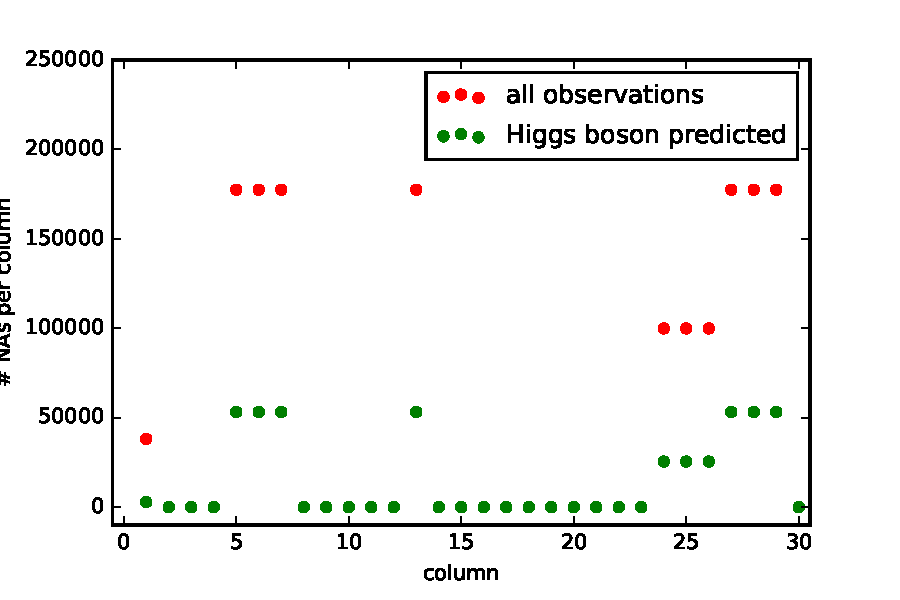
\includegraphics[width=\columnwidth]{Images/NAPerColumn.pdf}
  \caption{Number of NaN values in the data for each feature.}
  \vspace{-3mm}
  \label{fig:NaNsPerFeatures}
\end{figure}

Instead of removing the features with too many NaN values, we choose to replace them by the median of the values of the feature. The median is more robust than the mean. This improves over the method where no preprocessing at all is applied.

The interesting thing is that roughly $30\%$ of the provided data has a predicted Higgs boson, hence the trivial estimator can just assign "not predicted" to each data row which gives an overall prediction success of $70\%$. Hence, the benchline is to perform better than $70\%$ of correct predictions. With no preprocessing of the data at all (no replacement or removal of the data with NaN values), just standardizing the data to have zero mean and unit variance, we achieved $74\%$ of success (according to the Kaggle platform).

\subsection{Applying PCA}
Because the model becomes quite complex as the number of features increases, we implemented PCA (principal component analysis) to reduce the number of features. Choosing to keep a variance of $0.9999$ reduces the $30$ features to $15$ features. We further plotted histograms for each of the features that we kept to check they do not exhibit any odd behaviour or if anything is special that distinguishes data with the Higgs boson from the data without the Higgs boson. We also plotted the cross-dependence for each pair of features, but it is difficult for us to extract the features from the plots in an efficient way. In other words, we did not use these plots except for gross error checking. We did not notice anything special. See the ipynb notebook file for the plots or the "Images" directory in the same folder.


\subsection{Adding Polynomial Features Including Cross-Features}
We consequently added polynomial non-cross-related features and did cross-validation on them. But we thought that given the correlation figures we had produced before, there seemed some significant correlation. Hence, we programmed a method to also generate cross-features. For instance, for features $\{x, y\}$, we generate the features $\{1, x, y, x^2, xy, y^2, x^3, x^2y, xy^2, y^3\}$ up to degree $3$. We explicitly avoid duplicates $xy$ and $yx$, which would both be created in a naive approach, by relying on the unique factorization of primes (our own idea, see the code for this) to generate a mask that picks exactly one among $\{xy,yx\}$. In the program, we generate the cross-related features from degree $0$ to some degree $d_{\textrm{cross}}$ and then continue to generate the non-cross-related features from degree $d_{\textrm{cross}}+1$ to $d$. In a better approach, to avoid computation complexity and overfitting, one could bring in the patterns observed from the correlations graphs by eye, but this limits the systematic applicability of the model.

We are aware of the fact that the cross-related features introduce a lot more complexity to the model. To avoid overfitting, we rely on the cross-validation rejecting the overfitted models. Practically, we split the provided data into $5\%$ of training data and $95\%$ of testing data, which should be enough for detecting overfitted models.

\subsection{Using Cross-Validation to Select the Best Model}
As mentioned above, the most important is the model selection among the class of possible models using k-cross-validation with $k=5$. We also plotted the cross-validation error using the variance-bias decomposition from the exercises. The list of models has become quite large. Each generated model depends on the cross-feature degree $d_{cross}$, the polynomial degree $d$, the regularization parameter $\lambda$, which features to remove from the very start, the variance to keep for the PCA dimensionality reduction. Additionally, there is another loop to average over the seeds used to select the testing and training sets for cross-validation. We were forced to decide to remove some complexity. 

Changing one parameter at a time (ceteris paribus) and running cross-validation, we decided not to remove any features with too many NaN values and to keep $0.9999$ of the variance (total of 1) with PCA. With the NaN values, we achieved the best testing error estimates on the provided dataset, but scored worse on Kaggle. We interpret the removal of features as being too biased towards the provided data sample. What concerns the PCA, we were forced to reduce the dimensionality, so we thought, keeping $15$ features with a retained variance of $0.9999$ is still fine. For the seeds, we noticed that the training and testing errors do not change very much, so we restricted to two seeds (this is risky, but it takes too much time otherwise).

We also fixed the cross-feature degree to $d_{cross} = 3$, achieving best overall cross-validation results among all cross-features degrees. We checked this manually instead of putting a loop around it. In the code, we have the following loops: over the seeds, over the (non-cross-feature) degrees and over $\lambda$ (to select the best $\lambda$ for a given degree).

Due to the polynomial (cross and non-cross) features, our model has a lot of variables in the end and the prediction of the test file ('test.csv') for the Kaggle platform may encounter memory errors. That is why we are predicting and writing the data in chunks.

Finally, we always used the exact method to compute the weights (involving matrix inversion). We found that the direct method was faster than (stochastic) gradient descent and more reliable. For the cross-validation, we question whether it is good to select the method with least error or rather the method with best prediction accuracy (still using the least squares function for computing the weights).

\subsection{Applying Logistic Regression}
We also tried to apply logistic regression, but we did not get very good results with it. This time, there was no exact formula available and we had to use stochastic gradient descent, which we checked was better than pure gradient descent. To check the algorithm, we compared the computed gradient with the approximated gradient (using a central finite-difference formula) and we got quite different results. We cannot exclude errors although we checked several times. The reason the numerical gradient does not equal the analytical gradient might be computational inaccuracy due to small numbers, but we tried to pay attention to this by rewriting the involved sigmoid function $\sigma(x) = \frac{e^{-x}}{1+e^{-x}} = \frac{1}{1+e^{x}}$ and/or approximating $ln(1+e^x)\approx x$ for large $x \geq 10$.

\subsection{Possibility for Improvements and Outlook}
We obtained $81\%$ success with our method presented here, which is not that bad.
However, the machine learning approach to select the features appears very brutal to us. It was definitely a good idea to introduce cross-feature features, but greater care should be taken, which features to combine as this might significantly reduce the model complexity. We had another implementation of logistic regression (but forgot to commit it), where we achieved 80\%, which appears strange to us because logistic regression should be better.

With the polynomial features, we are for instance not able to capture a more complex relationship like an exponential or a logarithm. It would definitely prove useful to understand the physical significance of the provided measurements and develop an approximate parametrized physical model which we then fit with machine learning. In the end, we are not content with $81\%$ because we would at least need $99\%$ prediction accuracy because other indirect methods of detecting the Higgs boson are scarce.




%\bibliographystyle{IEEEtran}
%\bibliography{literature}

\end{document}
